\documentclass{standalone}
  \usepackage{tikz}
  \usetikzlibrary{arrows.meta, automata, bending, positioning, shapes.misc}
  \tikzstyle{automaton}=[shorten >=1pt, >={Stealth[bend,round]}, initial text=]

\begin{document}
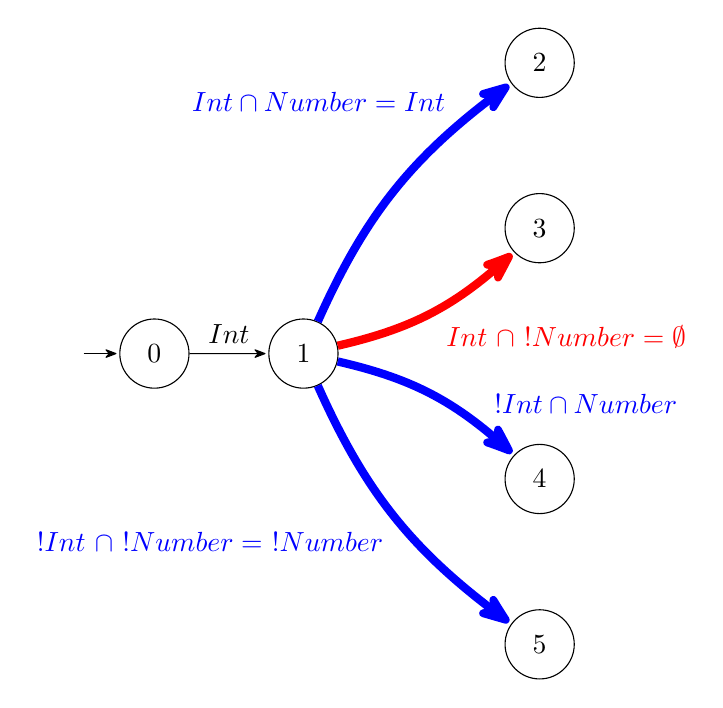
\begin{tikzpicture}[automaton, auto]
  \node[state,initial,rounded rectangle] (0) {$0$};
  \node[state,rounded rectangle] (1) [right=10mm of 0] {$1$};
  \node[state,rounded rectangle] (2) [above right=28mm and 30mm of 1] {$2$};
  \node[state,rounded rectangle] (3) [above right=7mm and 30mm of 1] {$3$};
  \node[state,rounded rectangle] (4) [below right=7mm and 30mm of 1] {$4$};
  \node[state,rounded rectangle] (5) [below right=28mm and 30mm of 1] {$5$};
  \path[->] (0) edge node {$Int$} (1);
  \path[->] (1) edge[blue, line width=3pt, bend left=15]  node[pos=.8] {$Int\cap Number = Int$} (2);
  \path[->] (1) edge[red, line width=3pt, bend right=15] node[swap] {$Int~\cap~ !Number = \emptyset$} (3);
  \path[->] (1) edge[blue, line width=3pt, bend left=15]  node[pos=.8] {$!Int \cap Number$} (4);
  \path[->] (1) edge[blue, line width=3pt, bend right=15] node[swap] {$!Int~ \cap~ !Number = ~ !Number$} (5);
\end{tikzpicture}
\end{document}
